\chapter{SNMP}

\section{Inleiding}

SNMP staat voor het Simple Network Management Protocol. De naam vertelt je meteen al waarvoor het protocol dient: het beheren van je netwerk.
De 'S' van SNMP betekent niet simpel als in simpel in gebruik (alhoewel het niet moeilijk in gebruik is), maar dat het protocol zo eenvoudig mogelijk gehouden is.
Met SNMP kun je allerhande informatie opvragen van verschillende soorten toestellen. In principe is er geen limiet op hetgeen je kunt opvragen van een toestel,
maar de functionaliteit om die informatie op te vragen moet wel geïmplementeerd worden. Normaal gezien gebeurt dat door de fabrikant van het toestel.

Er zijn maar een paar voorwaarden om met behulp van SNMP informatie van een toestel op te kunnen vragen. Eerst en vooral moet het toestel natuurlijk SNMP ondersteunen.
Ze moet ook de functionaliteit bezitten om de gevraagde informatie te kunnen aanbieden en tenslotte moet de vrager ook kennis hebben van welke informatie
er allemaal opgevraagd kan worden. Zo zal een router niet dezelfde informatie kunnen aanbieden als bijvoorbeeld een switch. Er is wel een minimale
verzameling van gegevens die door alle toestellen ondersteund moet worden om als SNMP-compatibel bestempeld te kunnen worden. Denk hierbij aan de naam van het
systeem, hoe lang het systeem al online is, welke netwerkinterfaces ze heeft, enzovoort.

Er zijn een groot aantal use cases te bedenken voor het gebruik van SNMP maar hier zijn enkele van de belangrijkste.

\begin{itemize}
	\item Inventarisatie: met behulp van discovery procedures en SNMP kun je een overzicht krijgen van alle toestellen aangesloten op het netwerk,
	en vooral hoe ze met elkaar verbonden zijn. Netwerken zijn niet statisch: er worden toestellen toegevoegd en verwijderd. Met SNMP kun je een
	actueel beeld van de aangesloten hardware en netwerktopologie verkrijgen. Dit is zeer handig voor kleine en middelgrote netwerken, maar onmisbaar
	voor grote netwerken!
	
	\item Configuratiebeheer: voor wat betreft de hardwarekant overlapt dit eigenlijk met de inventarisatie. Maar voor de softwarekant kun je met SNMP de
	configuratieinstellingen van toestellen opvragen en controleren. Bijvoorbeeld: voor Windowstoestellen kun je de lijst opvragen van geïnstalleerde updates,
	van routers kun je de routetabel controleren en van switches de \gls{arptabel}.
	
	\item Performantiebeheer: ook de netwerkverzadiging kun je controleren met SNMP. Zo kun je de huidige toestand in de gaten houden,
	onregelmatigheden vaststellen en trends volgen. Op basis van deze trends kunnen dan plannen opgesteld worden voor toekomstige uitbreidingen
	van de netwerkcapaciteit op knelpunten in het netwerk.
\end{itemize}

Voor kleine netwerken kan SNMP het leven van een systeembeheerder een stuk gemakkelijker maken. Om grote netwerken te beheren is SNMP quasi een vereiste.
De conclusie is duidelijk: SNMP zou onderdeel moeten uitmaken van de gereedschapskit van elke systeembeheerder.


% SNMP meer in detail / bouwstenen/onderdelen van SNMP
% Aspecten van SNMP?

\section{SNMP meer in detail}
\todo{Betere titel?}

\subsection{De S van SNMP}
\todo{Betere titel?}

Zoals gezegd staat de 'S' van SNMP voor simple. Hiermee wordt vooral bedoeld dat men SNMP zo simpel mogelijk heeft gehouden.
De reden waarom dit zo is, is tweeledig: eenvoud van implementatie en met oog op performantie. % Voor het toestel, niet het netwerk!!!
Omdat SNMP zo simpel in elkaar steekt, kunnen fabrikanten zonder al te veel moeite SNMP implementeren op hun hardware.
Door de simpliciteit van SNMP moet er bovendien slechts weinig werk verricht worden om SNMP-requests te beantwoorden.
Zodoende kunnen zelfs toestellen met zeer zwakke hardware, zoals embedded systemen, ook SNMP ondersteunen.


% Componenten?
\subsection{SNMP-toestelrollen}
\label{snmp-rollen}
\todo{Betere titel?}

SNMP kent twee soorten toestellen: \glspl{snmp-agent} en SNMP-managers.
In het client-server principe wordt de serverrol verricht door de \gls{snmp-agent} en de client door de SNMP-manager.

\begin{itemize}
	\item De \gls{snmp-agent} is een stuk software dat draait op de netwerkcomponenten en informatie bijhoudt over het toestel.
	Andere toestellen kunnen dan die gegevens opvragen en de \gls{snmp-agent} zal die aanvraag beantwoorden.
	
	% De GLS Reset zorgt ervoor dat de afkorting zeker languit wordt uitgeschreven
	\item De SNMP-manager, vaak een \glsreset{nms} \gls{nms} genoemd, is de software die de SNMP-requests genereert, verstuurt naar de
	\glspl{snmp-agent} en uiteindelijk de antwoorden verwerkt. Een \gls{nms} zal meestal niet één maar meerdere \glspl{snmp-agent} van verschillende toestellen ondervragen.
	Aan de hand van de verkregen informatie kan de \gls{nms} beslissen om verdere acties uitvoeren.
\end{itemize}


\subsection{Uniformiteit}
\todo{Betere titel?}

Een van de grootste voordelen van SNMP is het feit dat ze je een uniforme manier aanbiedt om je netwerk te beheren. Fabrikanten van netwerkapparatuur
bieden graag hun eigen oplossing aan om hun toestellen te beheren, maar het probleem is dat netwerken zelden uit apparatuur
bestaan van slechts een fabrikant. De managementoplossingen van de ene fabrikant werken natuurlijk niet om ook de toestellen van de andere
fabrikant te beheren. Met SNMP zit je dus niet vast aan een fabrikant en kun je op uniforme wijze gans je netwerk beheren.

SNMP biedt maar weinig functionaliteit aan en dat speelt zowel in zijn voordeel als in zijn nadeel.
Het voordeel is zoals eerder vermeld het gemak waarmee fabrikanten SNMP kunnen implementeren,
maar het nadeel is het gebrek aan features: met SNMP kun je enkel ruwe data opvragen.
Als je meer uit je data wenst te halen moet je die zelf achteraf verder verwerken. Denk aan het bijhouden van historische data, het combineren
van verschillende gegevens om verbanden te zien, grafieken opmaken of zelfs ganse rapporten opstellen. Die dingen worden wel ondersteund door de
managementoplossingen van fabrikanten, maar bij SNMP is het aan de gebruiker om die data uit de SNMP-gegevens te extraheren.


\subsection{Onderliggende protocols}

SNMP steunt op IP en UDP als transportprotocol. Dankzij de IP-laag kan SNMP ook werken op heterogene netwerken.
UDP werd verkozen boven TCP vanwege de eenvoudige werking, wat weer handig is voor low-level netwerkcomponenten.
Bovendien heeft UDP een kleinere impact op het netwerkverkeer dan TCP\cite{moreau}.
Het nadeel van UDP is wel dat er geen bevestiging gebeurt van verstuurde pakketten.
Als er een pakket verloren gaat is het dan aan de \gls{nms} om dit te detecteren en op te vangen.
Normaal zal een \gls{nms} simpelweg de SNMP-query opnieuw versturen.
Voor het versturen en ontvangen van SNMP-berichten wordt er standaard gebruik gemaakt van poort 161.


\section{Object Identifiers}

Elk mogelijk soort gegeven dat je kunt opvragen via SNMP van een toestel wordt wereldwijd uniek geïdentificeerd\cite{moreau} door een \gls{oid}.
\glspl{oid} worden hiërarchisch ingedeeld in een boomstructuur, net als bij DNS. De eindpunten van de boom stellen objecten voor en de knooppunten van de boom
worden gebruikt om objecten logisch te groeperen. De namen van de knooppunten bepalen de uiteindelijke \gls{oid}.
\glspl{oid} hebben een dotted-decimal notatie waarbij de knooppunten en het object van elkaar gescheiden worden door punten. %TODO Citatie?
Van links naar rechts wordt de \gls{oid} opgebouwd door het hoogste knooppunt tot het uiteindelijk object.
Een voorbeeld van een \gls{oid} die de uptime van een syteem teruggeeft is iso.org.dod.internet.mgmt.mib-2.system.sysUpTime.
Het stuk van de boomstructuur waarin die \gls{oid} valt kun je ook zien in \cref{boomstructuur}.

De tekstuele notatie van een \gls{oid} valt zoals je ziet nogal lang uit.
Daarom is het ook mogelijk om van een numerieke notatie gebruik te maken.
Elk knooppunt heeft behalve de tekstuele naam ook een volgnummer waar gebruik van kan gemaakt worden en een veel kortere \gls{oid} oplevert.
De \gls{oid} die hiervoor als voorbeeld werd gegeven wordt dan 1.3.6.1.2.1.1.3.
In de figuur van de boomvoorstelling staat het volgnummer van elk knooppunt ook tussen ronde haken. Eventueel kan er ook gebruik gemaakt worden van een
hybride notatie waarbij afwisselend gebruik kan gemaakt worden van de tekstuele of numerieke identificatie van een knooppunt.
Een mogelijke hybride voorstelling van het vorig voorbeeld is 1.3.6.1.mgmt.1.1.sysUpTime.

\begin{figure}[h]
	\centering
	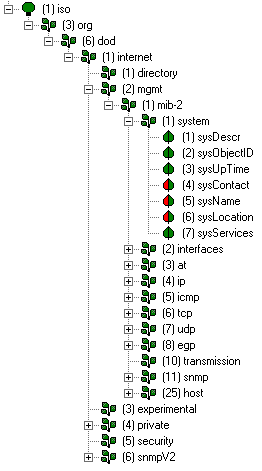
\includegraphics{figures/snmp/OID_tree}
	\caption{Boomstructuur van SNMP-objecten}
	\label{boomstructuur}
\end{figure}


\section{Management Information Base}
SNMP-agents houden een overzicht bij van alle gegevens die ze moeten bijhouden in een zogeheten \gls{mdb}.
In die \gls{mdb} zit een verzameling van \gls{mib} bestanden.\footnote{De \gls{mib}-bestanden worden eerst gecompileerd naar een binair formaat %TODO: Koppelteken?
alvorens ze in de \gls{mdb} opgeslagen worden.\cite{moreau}}
In die \gls{mib}-bestanden worden de eigenlijke SNMP-objecten gedefiniëerd. Vaak gaat men samenhorende objecten in een \gls{mib}-bestand samen stoppen.
Bijvoorbeeld alle objecten die bij een bepaald protocol horen, of alle objecten die worden geïmplementeerd door een bepaalde fabrikant.
Voor elk object wordt de naam en het volgnummer vastgelegd die zullen gebruikt worden in het OID voor dat object, alsook een beschrijving ervan en
van wat voor soort datastructuur er gebruik gemaakt wordt om de data voor te stellen (bv. een string of integer).

\begin{lstlisting}[language=asn.1, float=h, caption={Definitie van een SNMP-object}, label=lst-definitie-snmp-obj]
sysUpTime OBJECT-TYPE 
	 SYNTAX TimeTicks
	 ACCESS read-only
	 STATUS mandatory
	 DESCRIPTION "The time (in hundredths of a second) since the 
                  network management portion of the system was last 
                  re-initialized."
 	::= { system 3  }
\end{lstlisting}

Als voorbeeld kun je de definitie van hetzelfde \textit{sysUpTime}-object als eerder zien in \cref{lst-definitie-snmp-obj}.
Het \textit{ACCESS}-attribuut duidt hierbij aan of een gegeven gewijzigd mag worden of niet.
\textit{STATUS} geeft aan of het gegeven verplicht geïmplementeerd moet worden.
Onderaan zie je ook dat het object onder de \textit{system}-tak valt.

Ook voor \glspl{nms} zijn \gls{mib}-bestanden zeer belangrijk. Want ook zij moeten weten welke gegevens ze precies kunnen opvragen van een bepaalde
agent, en vooral: hoe ze die gegevens moeten interpreteren! Een \gls{nms} zal dus minstens \todo{minstens?} over dezelfde \glspl{mib} moeten beschikken als de
agents die hij ondervraagt. Een groot aantal \glspl{mib} zijn gestandaardiseerd en worden ook standaard meegeleverd met SNMP-software.
Een aantal van die gestandaardiseerde \glspl{mib} moeten ook verplicht ondersteund worden door SNMP-agents om de stempel 'SNMP compatibel' te mogen dragen.
Het MIB-2 knooppunt die je kunt zien in \cref{boomstructuur} is daar een voorbeeld van.
Die minimale set van gegevens zal je dus van ieder SNMP toestel kunnen opvragen.


\section{Tabellen}
\label{snmp-tabellen}

Behalve scalaire waarden is het ook mogelijk om tabellen op te vragen met SNMP.
We maken gebruik van de standaardtabel voor netwerkinterfaces \emph{ifTable} met als \gls{oid} 1.3.6.1.2.1.2.2 ter illustratie.
Een tabel wordt als volgt gedefiniëerd in een \gls{mib}-bestand: 
je hebt enerzijds een tabelobject (hier ifTable) en anderzijds een rijobject (hier ifEntry).
De definitie van het tabelobject zie je in \cref{definitie-iftable}.
De volgende codefragmenten tonen de definities van de overige objecten. %TODO: lstlistingname

Het tabelobject wordt gedefiniëerd als een sequentie of opeenvolging van rijobjecten.
Het rijobject wordt op zijn beurt gedefiniëerd als een sequentie van kolommen.
Hiervoor wordt een aparte sequentiedefinitie (IfEntry) gebruikt die 
bestaat uit een opeenvolging van kolomnamen gevolgd door hun datatype.

\begin{lstlisting}[language=asn.1, float=h, caption={Definitie van een tabel}, label=definitie-iftable]
ifTable OBJECT-TYPE
	SYNTAX	SEQUENCE OF IfEntry
	ACCESS	not-accessible
	STATUS	mandatory
	DESCRIPTION
			"A list of interface entries.  The number of
			entries is given by the value of ifNumber."
	::= { interfaces 2 }
\end{lstlisting}

\begin{lstlisting}[language=asn.1, float=h, caption={Sequentiedefinitie van een tabelrij}, label=definitie-sequentie-rij]
IfEntry ::=
	SEQUENCE {
		ifIndex
			INTEGER,
		ifDescr
			DisplayString,
		ifType
			INTEGER,
		...
	}
\end{lstlisting}

Bij de definitie van het rijobject zelf zie je dat er als syntax (datatype) de voorgaande sequentiedefinitie wordt gebruikt.
Merk op dat de sequentiedefinitie (IfEntry) begint met een hoofdletter maar de definitie van het object zelf niet (ifEntry).

\begin{lstlisting}[language=asn.1, float=h, caption={Definitie van een rijobject}, label=definitie-rijobject]
ifEntry OBJECT-TYPE
	SYNTAX	IfEntry
	ACCESS	not-accessible
	STATUS	mandatory
	DESCRIPTION
			"An interface entry containing objects at the
			subnetwork layer and below for a particular
			interface."
	INDEX	{ ifIndex }
	::= { ifTable 1 }
\end{lstlisting}

Ook belangrijk is het \textit{INDEX}-attribuut. Deze geeft aan hoe de tabel geïndexeerd moet worden, dus hoe je aan individuele rijen kunt geraken.
Dit kan een eenvoudige integer zijn of een samenstelling van kolommen die een rij uniek kan identificeren.
Hier wordt de index (ifIndex) gedefiniëerd als een eenvoudige integer.

\begin{lstlisting}[language=asn.1, float=h, caption={Definitie van een index}, label=definitie-ifindex]
ifIndex OBJECT-TYPE
	SYNTAX	INTEGER
	ACCESS	read-only
	STATUS	mandatory
	DESCRIPTION
			"A unique value for each interface.  Its value
			ranges between 1 and the value of ifNumber.  The
			value for each interface must remain constant at
			least from one re-initialization of the entity's
			network management system to the next re-
			initialization."
	::= { ifEntry 1 }
\end{lstlisting}

De indexering gebeurt dan als volgt. Om te beginnen heb je de \gls{oid} van de tabel zelf: 1.3.6.1.2.1.2.2.
Het rijobject heeft ook een eigen \gls{oid}. Zijn volgnummer is 1 dus die komt achter de \gls{oid} van de tabel.
Daarna komt het volgnummer van de kolom. Laten we als voorbeeld de kolom met de snelheid van de interface nemen (\textit{ifSpeed}).
Deze heeft als volgnummer 5. De \gls{oid} voor die kolom wordt dan 1.3.6.1.2.1.2.2.1.5.
Als we alle \glspl{oid} overlopen die beginnen met de \gls{oid} van de ifSpeed-kolom, dan krijgen we de waarden van alle rijen voor die ene kolom.
Als we ook nog eens een specifieke rij willen opgeven dan volgt dat na de kolomaanduiding.
Vermits er hier gebruik gemaakt wordt van een simpele integer als index kunnen we achteraan de \gls{oid} 1 toevoegen om 
de snelheid van de \emph{eerste} interface te weten te komen. De uiteindelijke \gls{oid} wordt dan 1.3.6.1.2.1.2.2.1.5.1.
Je kunt dit visueel ook bevestigen in \cref{boomstructuur-tabel,fig-tabel-oid}.

Omdat de kolomaanduiding voor de rijaanduiding komt in een \gls{oid},
zal het overlopen van alle \glspl{oid} die beginnen met de \gls{oid} van de tabel tot resultaat hebben dat de tabel kolom per kolom wordt overlopen.
Deze operatie wordt een SNMP walk van een \gls{oid} genoemd en wordt verder uitgelegd in \cref{snmp-getnext,snmp-walk}.

\begin{figure}[h]
	\centering
	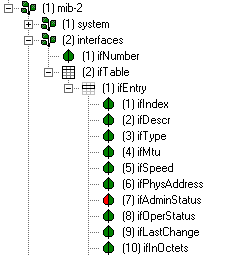
\includegraphics[resolution=110]{figures/snmp/ifTable-cropped}
	\caption{Boomstructuur van een tabel}
	\label{boomstructuur-tabel}
\end{figure}

\begin{figure}[h]
	\centering
	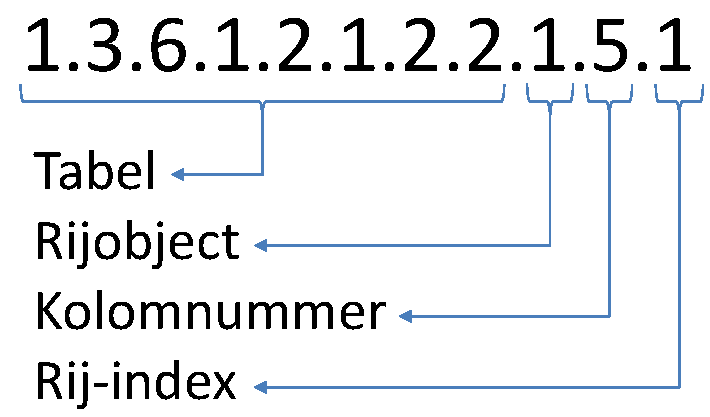
\includegraphics[scale=0.50]{figures/snmp/oid-tabel}
	\caption[OID van een cel uit een tabel]{\gls{oid} van een cel uit een SNMP-tabel}
	\label{fig-tabel-oid}
\end{figure}


\section{SNMP Operaties}
\label{snmp-operaties}
SNMP maakt gebruik van het \gls{pdu}-berichtformaat voor al het communicatieverkeer tussen SNMP-agents en \glspl{nms}.
Er worden een aantal verschillende operaties ondersteund door SNMP en die hebben elk hun eigen \gls{pdu}-formaat\cite{essentialsnmp}.
Hieronder worden enkel de belangrijkste SNMP-operaties gegeven die relevant zijn voor de masterproef:

\begin{itemize}
	\item GET
	\item GETNEXT
	\item GETBULK
\end{itemize}


\subsection{GET}
De GET-operatie was de eerste en belangrijkste SNMP operatie.
De GET-operatie wordt geïnitieerd door de \gls{nms} en laat die toe om een gegeven van een SNMP-agent op te vragen.
Om te weten welk gegeven de \gls{nms} nu juist wenst te weten te komen geeft die een \gls{oid} mee met de \gls{pdu} die het gegeven uniek zal identificeren.
Herinner je dat zowel de SNMP-agent als \gls{nms} over dezelfde \gls{mib} beschikken die dat \gls{oid} definiëert zodat ze beiden perfect weten waarover het gaat.
De SNMP-agent ontvangt de \gls{pdu} en verwerkt deze. Een nieuwe GET-response-\gls{pdu} wordt opgesteld voor dat \gls{oid} met de waarde ervan ingevuld en
teruggestuurd door de SNMP-agent. De \gls{nms} ontvangt de GET-response-\gls{pdu} en weet nu de waarde voor dat \gls{oid}.

\todo[inline]{Figuur?}


\subsection{GETNEXT}
\label{snmp-getnext}
De GETNEXT-operatie wordt gebruikt om een verzameling van opeenvolgende \glspl{oid} op te vragen.
Gegeven een bepaalde \gls{oid} zal de GETNEXT-operatie de eerstvolgende \gls{oid} met bijhorende waarde teruggeven.
Dit gebeurt in lexicografische volgorde en vermits \glspl{oid} samengesteld zijn door integers kan zo makkelijk een ganse boomtak overlopen worden.
Deze manier van werken noemt men diepte-eerst zoeken.\cite{essentialsnmp}
Wanneer de \gls{nms} het antwoord ontvangt van een GETNEXT-operatie zal ze een nieuwe sturen voor het volgende \gls{oid}.
De \gls{nms} zal blijven GETNEXT-\glspl{pdu} sturen tot dat de agent een foutmelding terugstuurt die aangeeft dat het einde van de \gls{mib} bereikt is.

De GETNEXT-operatie is vooral handig voor het overlopen van tabellen.
Tabellen zijn niet noodzakelijk sequentieel geïndexeerd, ze kunnen bijvoorbeeld samengesteld zijn aan de hand van een aantal attributen.
Maar met de GETNEXT-operatie hoef je daar geen rekening mee te houden, de GETNEXT-operatie geeft je meteen de volgende geldige index met de bijhorende gegevens.
De GETNEXT-operatie uitgevoerd op de OID van een tabel geeft je de eerste geldige index.
Daarmee kun je dan alle volgende indexen opvragen.

Normaal gezien zal je niet rechtstreeks in contact komen GETNEXT-operaties, maar zul je gebruik maken van de SNMP walkopdracht.
Je hoeft enkel de OID mee te geven met de SNMP walkopdracht waarop deze de nodige GETNEXT-requests zal sturen om de ganse boomtak te overlopen.
\todo{Herhaalt eigenlijk wat er hierboven werd gezegd, maar ipv NMS -> SNMP Walk}

\todo[inline]{Figuur?}


\subsection{GETBULK}
Met de tweede versie van SNMP werd de GETBULK-operatie gespecificeerd.
Deze operatie laat je toe om in een request meteen een heleboel \glspl{oid} op te vragen.
Bij een gewone GET-operatie kun je ook meerdere \glspl{oid} meegeven maar de berichtgrootte wordt beperkt door de capaciteit van de SNMP-agent.
Als een SNMP-agent geen antwoord kan geven op alle \glspl{oid} die werden gevraagd in de GET-operatie wordt een foutboodschap teruggestuurd zonder data.
De GETBULK-operatie daarentegen probeert zo veel mogelijk data terug te sturen als het kan.
Met de GETBULK-operatie is het dus wel mogelijk om incomplete antwoorden terug te krijgen.\cite{essentialsnmp}

\section{Manieren om SNMP gegevens op te vragen}
\label{manieren-om-snmp-gegevens-op-te-vragen}

Aan de hand van de SNMP-operaties besproken in \cref{snmp-operaties} zijn er verschillende mogelijkheden om gegevens op te vragen
al naar gelang je een of meerdere gegevens wenst op te vragen en welke gegevens \todo{Sequentiele gegevens?} je juist wenst op te vragen (bv. tabellen).
Met behulp van Net-SNMP zullen de verschillende mogelijkheden hieronder gedemonstreerd worden.
Net-SNMP is een gratis en open-source softwarepakket die commando's aanbiedt voor de verschillende SNMP-operaties en
is beschikbaar voor de meeste besturingssystemen waaronder Windows en Linux.
Wij maken gebruik van de Linux versie.


\subsection{Een gegeven}
%TODO: Goede titel? Enkelvoudig/meervoudig? Een/meerdere gegevens?

\subsubsection{GET-operatie}

Indien je maar geïnteresseerd bent in slechts een gegeven dan ligt het voor de hand om gebruik te maken van de SNMP GET-operatie.
Voorwaarde is wel dat je exact de \gls{oid} kent van het gegeven dat je wenst op te vragen.
Een GET-request in Net-SNMP ziet er zo uit:

\begin{lstlisting}[float=h, caption={SNMP GET-opdracht}, label=netsnmp-get]
$ snmpget -v 1 -c public 127.0.0.1 sysDescr.0
SNMPv2-MIB::sysDescr.0 = STRING: Linux debian-vm-01 3.2.0-4-amd64 #1 SMP Debian 3.2.54-2 x86_64
\end{lstlisting}

Daarbij geeft de -v optie de te gebruiken versie mee en de -c optie de \textit{communitystring}.
De communitystring fungeert als een soort wachtwoord om SNMP-requests te beveiligen.
De opties worden gevolgd door het IP adres van het te ondervragen toestel en het \gls{oid} van het gegeven dat je wenst op te vragen.
Zoals je misschien al opgemerkt hebt, wordt de \gls{oid} hier niet voorafgegaan door iso.org.dod.internet.mgmt.mib-2.system zoals het zou horen
voor een \gls{oid} die in die subtak valt. De reden daarvoor is dat dit niet vereist is als de naam van de tak uniek is, wat het geval is voor sysDescr.

De volgende vraag die je wellicht stelt is waarom er nog een .0 achter de \gls{oid} staat.
Dit is omdat MIB objecten geïdentificeerd worden door de conventie x.y waarbij x de \gls{oid} is van het object
en y de instantie aanduidt. Normaal wordt y gebruikt bij tabellen om de rij aan te duiden (1 is de eerste rij, 2 de tweede, enzovoort),
zoals uitgelegd in \cref{snmp-tabellen}.
Maar bij scalaire objecten is y altijd 0. De .0 achterwege laten levert een fout op.\cite{essentialsnmp}

\subsubsection{GETNEXT-operatie}

Je kan ook gebruik maken van de SNMP GETNEXT-operatie als je het \emph{volgende} gegeven wenst te weten te komen.
Dit wordt hoofdzakelijk gebruikt bij het overlopen van tabellen zonder dat je moet rekening houden met de indexering van de tabel
die niet noodzakelijk sequentieel is.
Het is mogelijk om zelf een SNMP GETNEXT-operatie uit te voeren, maar normaliter maak je gebruik van de SNMP walkopdracht die
hiervan gebruik maakt om een ganse boomtak te overlopen. Hier gaan we verder op in in \cref{snmp-getnext}.

Als je de indexering van een tabel niet kent, dan zou je het volgende kunnen doen:

\begin{lstlisting}[float=h, caption={SNMP GETNEXT-opdracht op een tabel}, label=netsnmp-getnext]
$ snmpgetnext -v 1 -c public 127.0.0.1 ifTable
IF-MIB::ifIndex.1 = INTEGER: 1
\end{lstlisting}

Dit levert dan de waarde van de eerste kolom (hier ifIndex) van de eerste rij op.
Herinner je dat de \gls{oid} van een tabelelement eerst het kolomnummer bevat en dan de index van de rij.
Dus als je de waarde van een andere kolom wenst zonder dat je de index van de eerste rij kent, zou je het volgende kunnen doen:

\begin{lstlisting}[float=h, caption={SNMP GETNEXT-opdracht op een kolom van een tabel}, label=netsnmp-getnextcol]
$ snmpgetnext -v 1 -c public 127.0.0.1 ifTable.1.2
IF-MIB::ifDescr.1 = STRING: lo
\end{lstlisting}

Dit levert dan de tweede kolom (de beschrijving van de interface, hier lo, kort voor loopback interface) op van de eerste rij.
Maar zoals gezegd zul je eerder gebruik maken van de SNMP walkopdracht dan GETNEXT-operaties (zie verder).


\subsection{Meerdere gegevens}

\subsubsection{SNMP BULK-operatie}
Als je meerdere gegevens wenst op te vragen gebruik je best de SNMP BULK-operatie.
Deze combineert meerdere \glspl{oid} in een bericht waardoor je sneller meerdere gegevens kunt opvragen.
In feite zal de SNMP BULK-operatie simpelweg meerdere GETNEXT-operaties uitvoeren en de resultaten combineren in een bericht.

Om van SNMP BULK-operaties gebruik te maken moet je ten eerste zorgen dat je gebruik maakt van SNMP versie 2c
(zie ook \cref{snmp-versies} waarin we de verschillende SNMP versies bespreken).
Ten tweede moet je ook twee extra parameters opgeven: \textit{non-repeaters} en \textit{max-repetitions}.
Je kunt meerdere \glspl{oid} meegeven met de BULK-operatie en met die parameters kun je opgeven of er slechts een keer
een GETNEXT-operatie op een \gls{oid} moet uitgevoerd worden of meerdere.
Non-repeaters geeft aan hoeveel \glspl{oid} er zijn meegegeven waarop slechts een keer een GETNEXT-operatie moet uitgevoerd worden.
Deze \glspl{oid} zullen dus elk slechts een antwoord bevatten in het antwoordbericht.
Met max-repetitions geef je aan hoeveel keer er een GETNEXT-operatie moet uitgevoerd worden op de overige \glspl{oid}.
Als je max-repetitions op 10 zet, dan zal je voor elk van de overige \glspl{oid} 10 antwoorden krijgen in het antwoordbericht.
Vermits je enkel opgeeft hoeveel \glspl{oid} niet herhalen (non-repeaters) moet je eerste de niet-herhalende \glspl{oid} opgeven en dan de herhalende.
Wellicht dat een voorbeeld meer duidelijkheid verschaft:

\begin{lstlisting}[float=h, caption={SNMP BULK-opdracht}, label=netsnmp-bulk]
$ snmpbulkget -v 2c -c public -Cn1 -Cr3 127.0.0.1 sysDescr ifTable ipAddrTable
SNMPv2-MIB::sysDescr.0 = STRING: Linux debian-vm-01 3.2.0-4-amd64 #1 SMP Debian 3.2.54-2 x86_64
IF-MIB::ifIndex.1 = INTEGER: 1
IP-MIB::ipAdEntAddr.10.0.2.11 = IpAddress: 10.0.2.11
IF-MIB::ifIndex.2 = INTEGER: 2
IP-MIB::ipAdEntAddr.127.0.0.1 = IpAddress: 127.0.0.1
IF-MIB::ifIndex.3 = INTEGER: 3
IP-MIB::ipAdEntIfIndex.10.0.2.11 = INTEGER: 2
\end{lstlisting}

Het aantal non-repeaters en het aantal max-repetitions worden ingesteld met respectievelijk de -Cn en de -Cr optie.
Vermits het aantal non-repeaters op 1 staat wil dit zeggen dat enkel de eerste \gls{oid}, sysDescr, niet herhaald moet worden.
En omdat max-repetitions op 3 staat, worden alle overige \glspl{oid} drie keer herhaald (hier ifTable en ipAddrTable).
Als antwoord zie je het volgende staan: de waarde van sysDescr, de eerste drie waarden van ifTable en de eerste drie waarden van ipAddrTable.

Merk op dat de versie nu op 2c staat. Verder zie je dat de \gls{oid} voor de scalaire waarde sysDescr nu niet gevolgd wordt door .0,
want achterliggend maakt de BULK-operatie gebruik van een GETNEXT-operatie.
Als je toch .0 toevoegt dan zul je niet de waarde van sysDescr terugkrijgen maar die van de volgende \gls{oid}.
Moest je ten slotte een hoger aantal max-repetitions gebruiken dan een tabel cellen heeft,
of per ongeluk een scalaire waardere meerdere keren laten herhalen, dan krijg je ook nog de waarden van de \glspl{oid} die volgen op de tabel of de scalaire waarde terug.
\todo[inline]{Te verwarrend?}


\subsubsection{GET- en GETNEXT-opdrachten}
\label{meerdere-gegevens-ophalen-met-GET-en-GETNEXT}

In principe is het ook mogelijk om meerdere gegevens op te vragen met een GET- of GETNEXT-opdracht.
Om dat te doen geef je simpelweg meerdere \glspl{oid} mee in de opdracht:

\begin{lstlisting}[float=h, caption={Meerdere gegevens opvragen met SNMP GET}, label=netsnmp-get-meerdere]
$ snmpget -v 1 -c public 127.0.0.1 sysDescr.0 sysUpTime.0 sysName.0
SNMPv2-MIB::sysDescr.0 = STRING: Linux debian-vm-01 3.2.0-4-amd64 #1 SMP Debian 3.2.54-2 x86_64
DISMAN-EVENT-MIB::sysUpTimeInstance = Timeticks: (1451759) 4:01:57.59
SNMPv2-MIB::sysName.0 = STRING: debian-vm-01
\end{lstlisting}

Het nadeel van dit te doen met een GET- of GETNEXT-opdracht is dat, als er een fout optreedt bij het opvragen
van een van de \glspl{oid}, je geen gegevens terug zal krijgen over de \glspl{oid} die wel correct waren:

\begin{lstlisting}[float=h, caption={Meerdere gegevens opvragen met SNMP GET met een foute OID}, label=netsnmp-get-meerdere-fout]
$ snmpget -v 1 -c public 127.0.0.1 sysDescr.0 sysUpTime.0 sysName.0 fouteOID
fouteOID: Unknown Object Identifier (Sub-id not found: (top) -> fouteOID)
\end{lstlisting}

Bij een BULK-opdracht krijg je die gegevens wel.
Om meerdere gegevens op te vragen maak je dus beter gebruik van BULK-opdrachten.


\subsubsection{SNMP walk}
\label{snmp-walk}

Zoals gezegd maak je normaal gezien weinig gebruik van de GETNEXT-operatie maar gebruik je in de plaats de SNMP walkopdracht.
De SNMP walkopdracht wordt gebruikt om een ganse boomtak te overlopen en maakt achterliggend gebruik van GETNEXT-operaties.
Met de volgende SNMP walkopdracht kun je de interfacetabel van een toestel overlopen:

\begin{lstlisting}[caption={SNMP walkopdracht}, label=netsnmp-walk]
$ snmpwalk -v 1 -c public 127.0.0.1 ifTable
IF-MIB::ifIndex.1 = INTEGER: 1
IF-MIB::ifIndex.2 = INTEGER: 2
IF-MIB::ifIndex.3 = INTEGER: 3
...
IF-MIB::ifSpecific.4 = OID: SNMPv2-SMI::zeroDotZero
IF-MIB::ifSpecific.5 = OID: SNMPv2-SMI::zeroDotZero
IF-MIB::ifSpecific.6 = OID: SNMPv2-SMI::zeroDotZero
\end{lstlisting}

Merk op dat we hier geen instantie (de .0 bij scalaire gegevens) na de \gls{oid} hebben opgegeven!
Moest je hier toch een instantie opgeven (de index van een rij van de tabel) dan zou je slechts een kolomwaarde terugkrijgen,
horende bij die rij en had je hetzelfde kunnen bereiken met een SNMP GET-opdracht.
\todo[inline]{Verwarrend?}

Vermits BULK-operaties ook gebruik maken van GETNEXT-operaties, maar die bundelen in een antwoord,
kun je de SNMP walkopdracht nog sneller laten verlopen door de BULK-variant te gebruiken.
Het resultaat blijft natuurlijk hetzelfde.

\begin{lstlisting}[caption={SNMP walkopdracht m.b.v. BULK-operaties}, label=netsnmp-bulkwalk]
$ snmpbulkwalk -v 2c -c public 127.0.0.1 ifTable
...
\end{lstlisting}

Let erop dat je de versie moet veranderen omdat je gebruik maakt van BULK-operaties!

Net als bij het snmpbulkget-commando kun je hier echter nog het aantal herhalingen (max-repetitions) opgeven met de -Cr optie.
Daarbij komt het erop neer dat we kunnen opgeven hoeveel objecten moeten samengebundeld worden in een pakket.
Om een SNMP walk zo snel mogelijk te laten verlopen zijn we natuurlijk geneigd om dit aantal zo hoog mogelijk in te stellen.
We moeten echter wel rekening houden met een aantal zaken.
Ten eerste is de maximale grootte van een pakket beperkt tot de \gls{mtu} van een verbinding.
Bij een ethernetverbinding gaat het om 1500 Bytes.

Ten tweede is het bij een groot aantal herhalingen ook mogelijk dat er redelijk wat data verspild wordt.
Stel dat we het aantal herhalingen instellen op 50, dan zullen de pakketten steeds 50 objecten bevatten.
Ook het laatste pakket zal er 50 bevatten, ook al valt er slechts een object meer binnen de walk.
Dan zijn de overige 49 objecten natuurlijk niet relevant voor ons en doen we daar dan ook niks mee.

Als we een walk doen van een deelboom die maar 10 objecten heeft, heeft het ook geen zin om het aantal herhalingen op 50 te zetten.
Natuurlijk weet je op voorhand niet hoeveel objecten juist onder een \gls{oid} vallen,
maar je kan meestal wel een schatting doen of dit baseren op het aantal objecten dat in het verleden werd opgehaald voor dat \gls{oid} van een bepaald toestel.

Het aantal herhalingen is uiteindelijk een beslissing die vooral zal afhangen van het geschatte aantal gegevens dat opgevraagd gaat worden.
Standaard staat het aantal herhalingen daarom op een conservatieve 10 objecten.


\section{Versies}
\label{snmp-versies}
Er zijn drie grote versies van SNMP die momenteel in gebruik zijn op netwerktoestellen: SNMPv1, SNMPv2c en SNMPv3.
Ondanks dat SNMPv3 de twee voorgaande versies opvolgt kun je nog steeds veel toestellen vinden die enkel met SNMPv2c of zelfs met SNMPv1 werken.
Het is aan de fabrikant om voor de ondersteuning van SNMPv3 te zorgen op een toestel.


\subsection{SNMPv1}
De eerste versie van SNMP dateert al van 1988 maar is soms toch nog te vinden als enige ondersteunde versie op een toestel.
Een van de grootste gebreken die deze versie kenmerkt is de beveiliging.
De originele versie van SNMP maakte gebruik van een zogeheten \emph{community string} om SNMP-requests te beveiligen.
Die string fungeerde in feite als een soort wachtwoord die in cleartext met ieder SNMP-request werd meegegeven\cite{snmp-wiki}.
Natuurlijk kan iedereen die de requests kan onderscheppen het wachtwoord gewoon uitlezen en zelf requests met dat wachtwoord versturen.
SNMP voorziet in de mogelijkheid om niet alleen data uit te lezen, maar ook om data aan te passen met behulp van de SNMP SET-operatie.
Vanwege de slechte beveiliging wordt de SET-operatie echter zo goed als nooit geïmplementeerd in de SNMP-agent zodat de operatie geen effect heeft.

\todo[inline]{Waarom werd deze versie geaccepteerd? Werd aanzien als tijdelijke oplossing.}


\subsection{SNMPv2c}
De tweede versie van SNMP introduceerde in 1993 \cite{snmp-versions} oorspronkelijk de GETBULK-operatie en een betere beveiliging.
De nieuwe beveiliging werd echter als te complex beschouwd en werd op veel plaatsen niet aanvaard.
SNMPv2c werd in 1996 \cite{snmp-versions} voorgesteld als een alternatief die de verbeteringen van SNMPv2 had maar de complexe beveiliging ervan achterwege liet
ten voordele van de community strings van SNMPv1.
Deze versie werd wel aanvaard door de gemeenschap en is nog steeds in gebruik op een groot aantal toestellen.
De GETBULK-operatie was een welkome toevoeging aan SNMP omdat ze een veel performanter alternatief bood voor de vele GETNEXT-operaties
die voorheen nodig waren om grote hoeveelheden gegevens op te vragen.

\todo[inline]{Cross-compatibility met vorige versie}


\subsection{SNMPv3}
De derde en laatste versie van SNMP werd geaccepteerd als een volwaardige internetstandaard in 2002 \cite{snmpv3} en
bracht de reeds lang gevraagde verbetering in beveiliging met zich mee.
Omdat de vorige versies van SNMP slecht beveiligd waren werd het protocol enkel gebruikt voor het monitoren van het netwerk en performantiebeheer.
Met de verbeterde beveilging in SNMPv3 kan SNMP eindelijk een veilig platform aanbieden om niet enkel je netwerk passief te beheren zoals voorheen,
maar ook actief te beheren door configuratiewijzigingen uit te voeren via SNMP.
SNMPv3 is echter op veel toestellen nog steeds niet aanwezig en zeker de SNMP SET-operatie wordt in de praktijk maar zelden geïmplementeerd.

\section{Berichtstructuur van SNMP}
\label{snmp-berichtstructuur}

In deze paragraaf bespreken we de berichtstructuur van een SNMP-bericht.
In tegenstelling tot bijvoorbeeld IP- en ethernetheaders, hebben de headers van SNMP-berichten geen vaste lengte.
In de plaats daarvan bestaat een SNMP-bericht uit \gls{tlv} tripletten\cite{moreau}.
Daarbij geeft de tag aan om wat voor datatype het gaat, length duidt de lengte aan van de data en value bevat de data zelf.
Je hebt primitieve datatypes zoals een integer, een octetstring of een \gls{oid}.
Maar je hebt ook complexe datatypes zoals een sequentie of een \gls{pdu} voor bijvoorbeeld een GET-request of een GET-response.
De complexe types zoals de sequentie zijn opgebouwd uit meerdere kleinere velden zodat je een geneste structuur krijgt\cite{snmp-message-format}.

\begin{table}[h]
\centering
\begin{tabular}{@{}ll@{}}
\toprule
Primitieve datatypes & Complexe datatypes \\ \midrule
Integer              & Sequence           \\
Octet String         & GetRequest         \\
Object Identifier    & GetResponse        \\
Null                 & GetBulkRequest     \\ \bottomrule
\end{tabular}
\caption{Enkele SNMP-datatypes}
\label{tabel-datatypes}
\end{table}

Een SNMP-bericht is dus niks meer dan een geneste structuur van datavelden.
Het SNMP-bericht zelf wordt gedefinieerd als een sequentie van drie velden: een integer die de SNMP versie voorstelt, een octetstring die de community voorstelt en
de eigenlijke SNMP-\gls{pdu} (zelf een samengesteld type).

\begin{figure}[h]
	\centering
	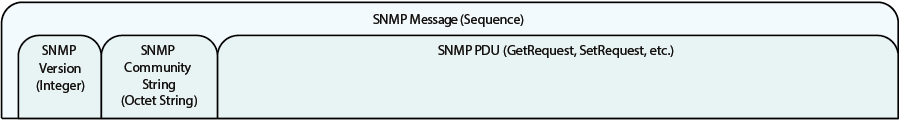
\includegraphics[scale=0.45]{figures/snmp/berichtstructuur-1}
	\caption[Berichtstructuur van een SNMP-bericht]{Berichtstructuur van een SNMP-bericht\cite{snmp-message-format}}
	\label{fig-berichtstructuur-1}
\end{figure}

De SNMP-\gls{pdu} bestaat uit de volgende velden:

\begin{itemize}
	\item Request ID (integer): een unieke identificatie van een SNMP-request.
		Het responsbericht zal dezelfde identificatie gebruiken zodat de ontvanger weet bij welke request het antwoord hoort.
	\item Error (integer): duidt aan of er een fout is opgetreden.
		De SNMP-agent zal deze waarde veranderen indien nodig. Als de waarde op nul staat is er geen fout opgetreden.
	\item Error Index (integer): verwijst naar het object dat de fout heeft veroorzaakt.
	\item Varbind List (sequentie): de verzameling van alle objecten in de \gls{pdu}.
		\begin{itemize}
			\item Varbind (sequentie): komt overeen met een object en bevat zijn \gls{oid} en waarde.
				De waarde wordt enkel ingevuld in het responsbericht.
				\begin{itemize}
					\item Object Identifier (OID)
					\item Value (integer, octetstring, \ldots)
				\end{itemize}
		\end{itemize}
\end{itemize}

\begin{figure}[h]
	\centering
	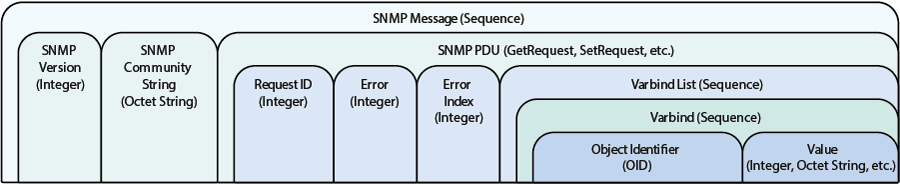
\includegraphics[scale=0.45]{figures/snmp/berichtstructuur-2}
	\caption[Berichtstructuur van een SNMP-bericht en zijn SNMP-PDU]{Berichtstructuur van een SNMP-bericht en zijn SNMP-\gls{pdu}\cite{snmp-message-format}}
	\label{fig-berichtstructuur-2}
\end{figure}

Een voorbeeld van een GET-request in detail zie je in \cref{fig-berichtstructuur-3}.
Onderaan zie je de hexadecimale waarden van de bytes.
De eerste byte van een veld duidt steeds de code van het datatype aan en de tweede de lengte van het veld.
De volgende bytes vormen dan de inhoud van het veld.
Zodoende krijgen we de Tag-Length-Value tripletten waar we over spraken.
Merk op dat als de lengte van een veld verandert dat deel uitmaakt van een complex datatype zoals een sequentie,
dan moet de lengte van het bovenliggende datatype ook aangepast worden.

Omdat het hier om een request gaat, is de waarde van het object nog niet ingevuld.
Daarmee zien we meteen ook het doel van het Null-datatype: zo kan er aangegeven worden dat een veld niet is ingevuld en kan er een byte uitgespaard worden.
De value van het \gls{tlv}-triplet is dan ook niet aanwezig en zijn lengte is nul.

\begin{figure}[h]
	\centering
	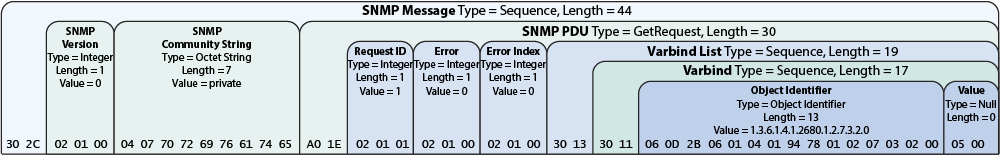
\includegraphics[scale=0.40]{figures/snmp/berichtstructuur-3}
	\caption[Berichtstructuur van een SNMP-bericht in detail]{Berichtstructuur van een SNMP-bericht in detail\cite{snmp-message-format}}
	\label{fig-berichtstructuur-3}
\end{figure}